\begin{simulation}
\label{sim::zebra} 
\end{simulation}

\noindent Considere o manipulador antropom�rfico Zebra-ZERO (Ap�ndice \ref{ap::zebra}), e o rastreamento de posi��o do punho (trajet�ria \ref{traj}) e regula��o da orienta��o (${\bf R}_d = {\bf R}_y(\pi/2)$). A seguir, s�o apresentados resultados de simula��o obtidos para ${\boldsymbol \Lambda}_p = {\boldsymbol \Lambda}_o = 5\,{\bf I}$.

\begin{figure}[!htp]
			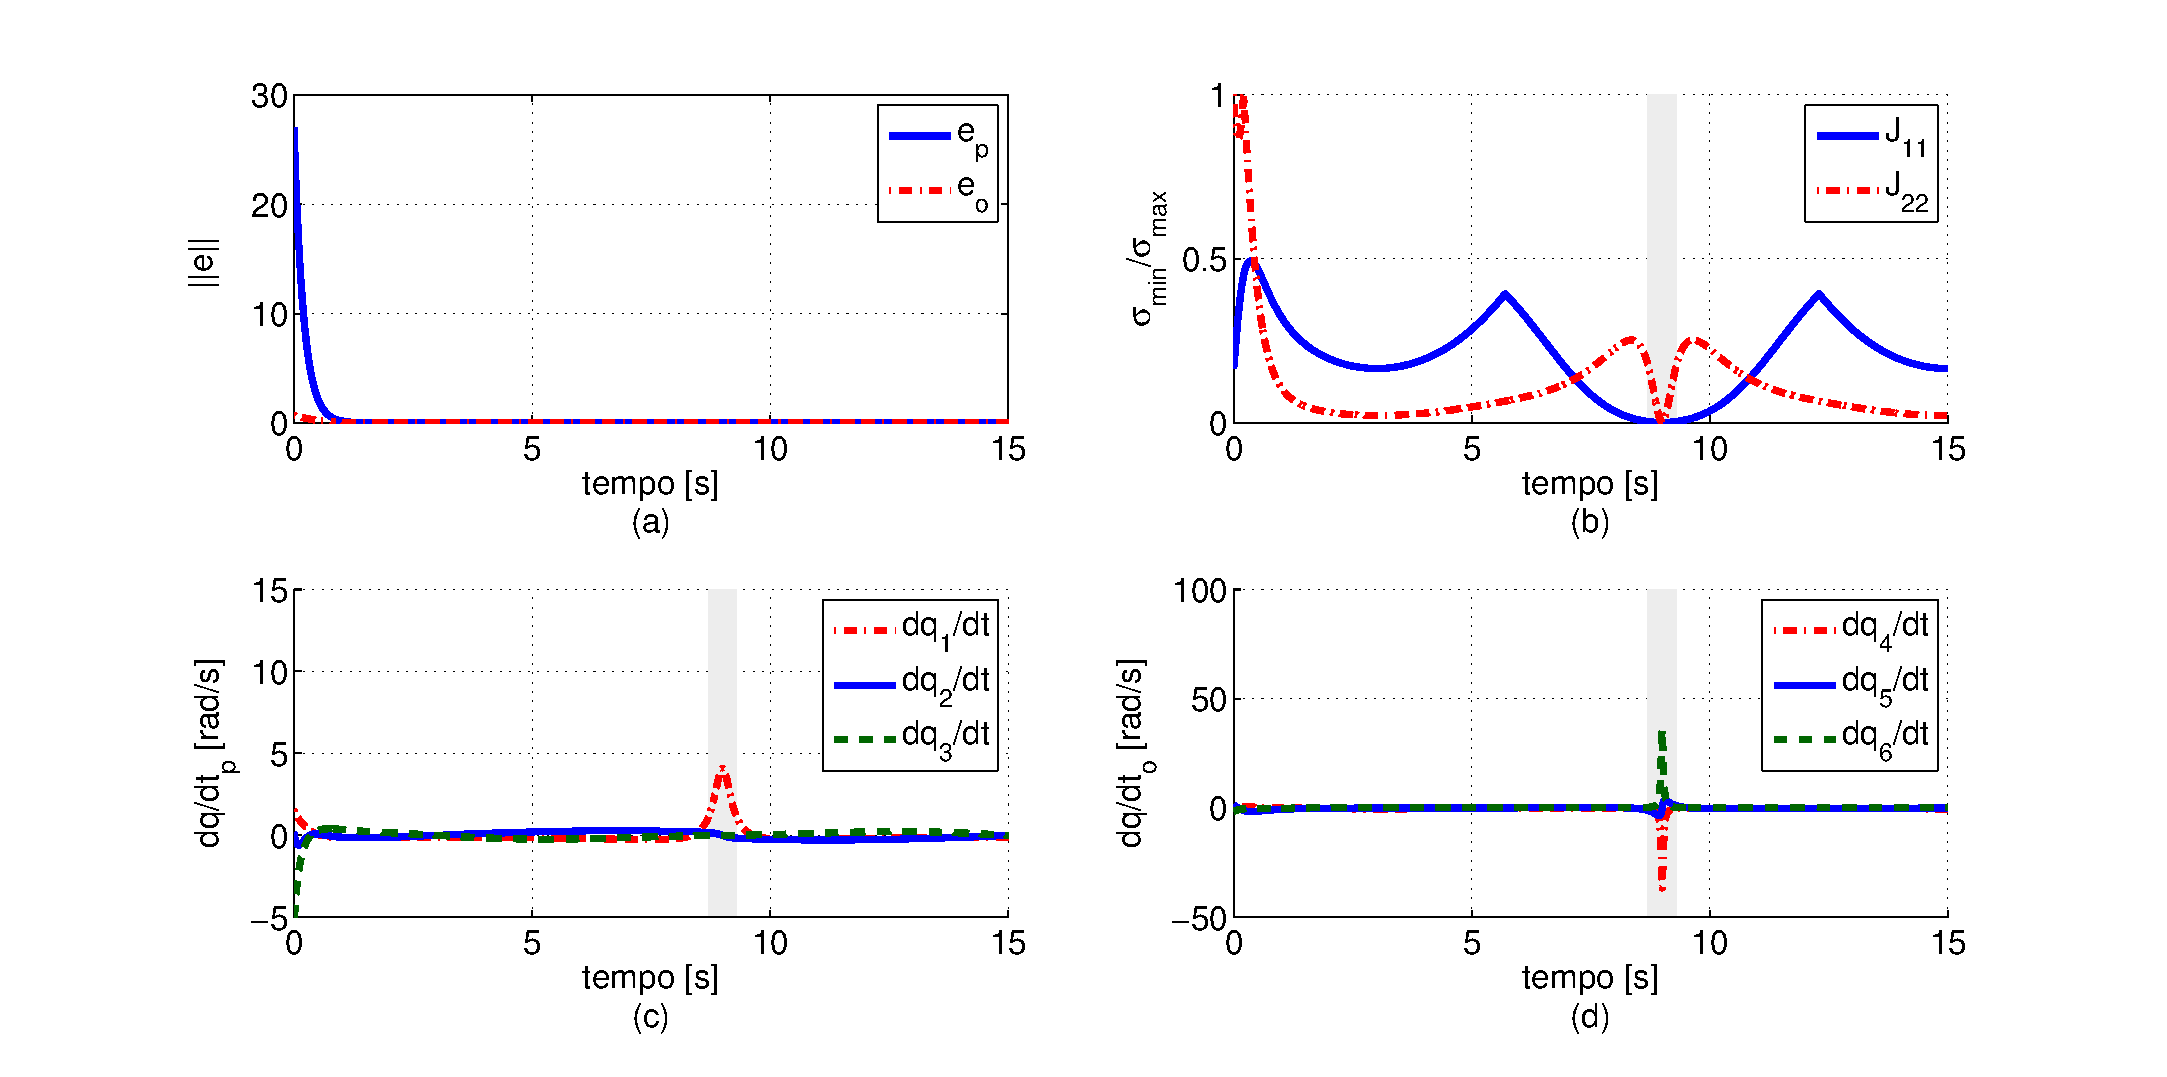
\includegraphics[trim = 2.7cm 1.2cm 2.7cm 0.5cm, scale = 0.49]{sim/simzebra_data.eps}\\
			%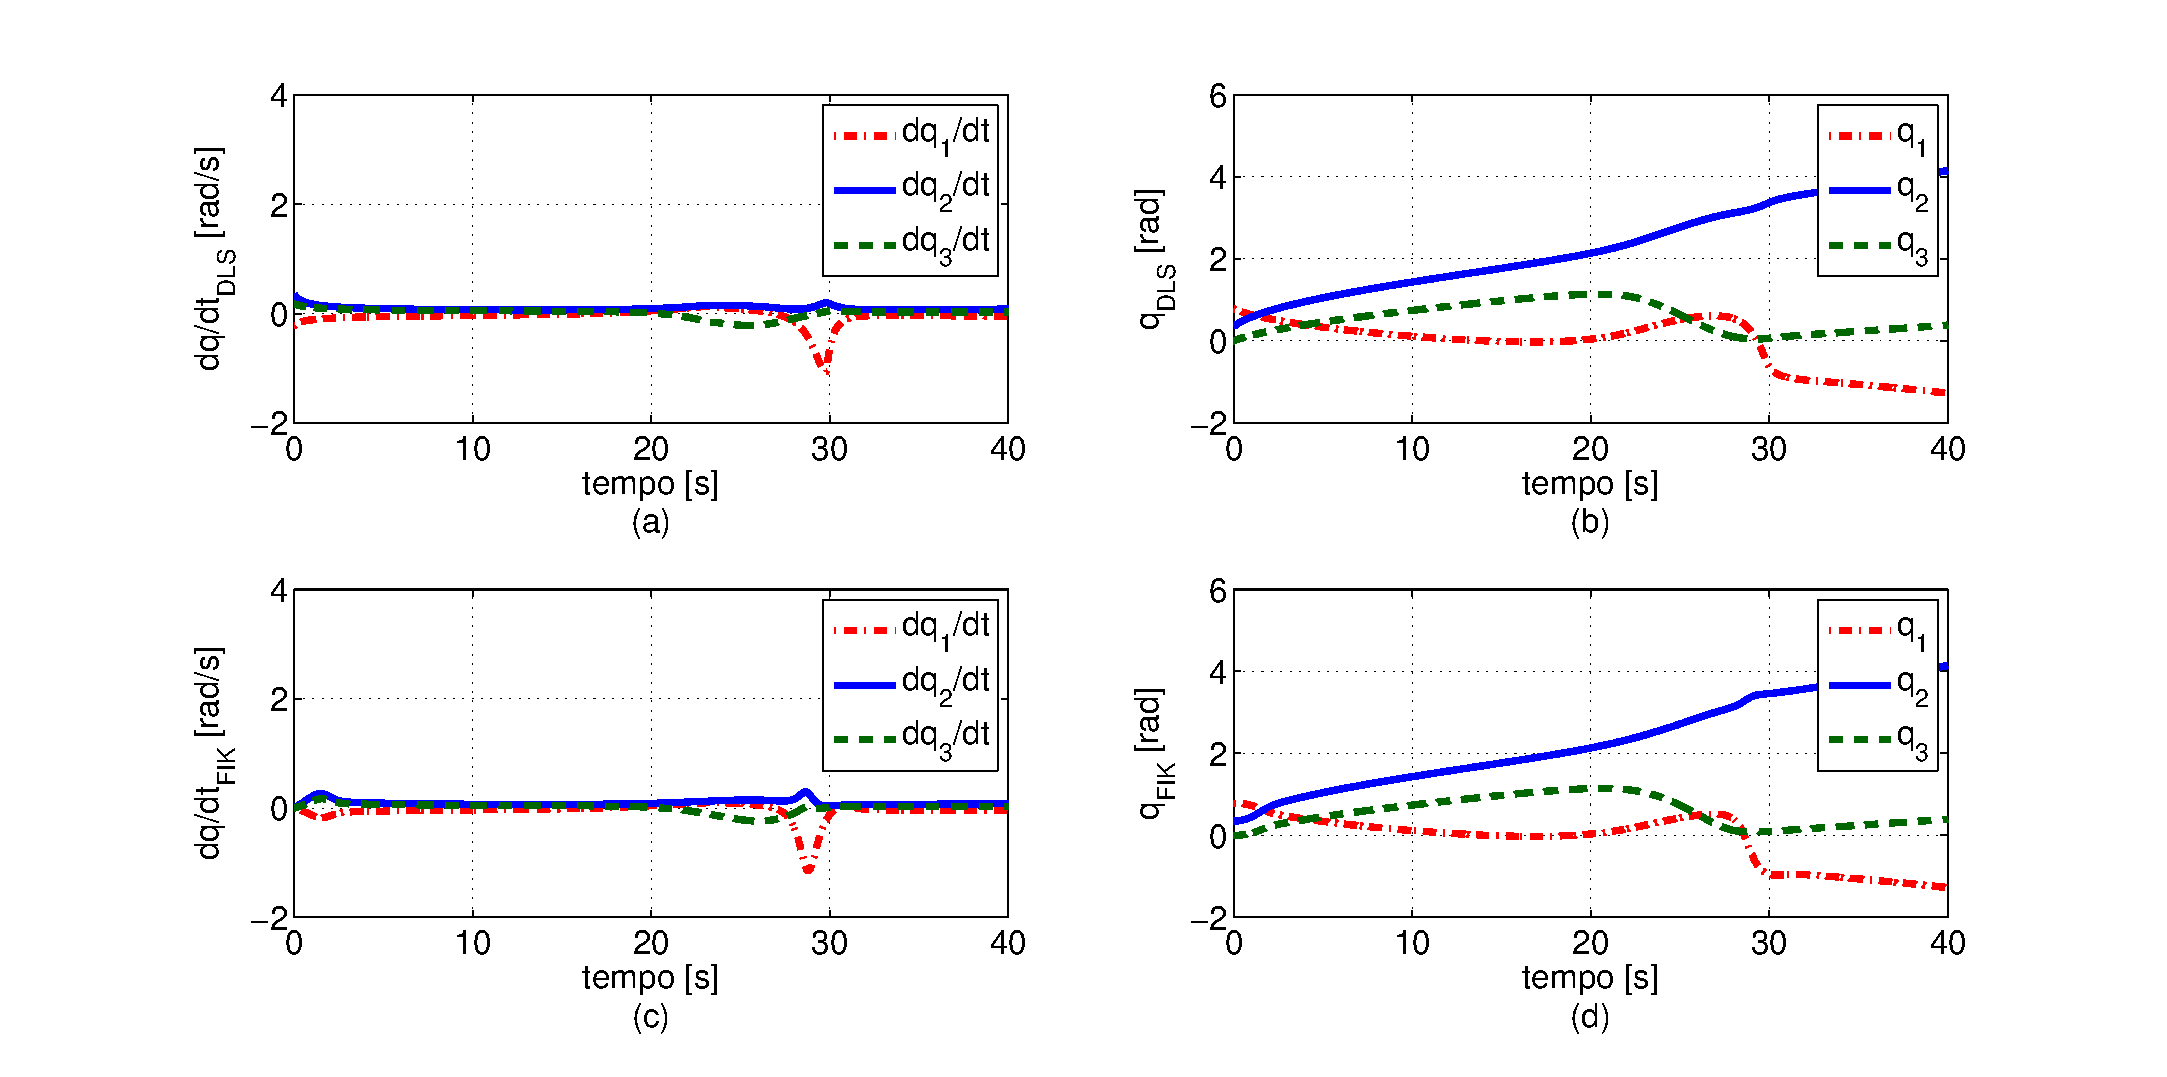
\includegraphics[trim = 2.7cm 10cm 2.7cm 1cm, scale = 0.49]{sim/sim3_data2.eps}\\ %\tiny{\,(b)} \\
			%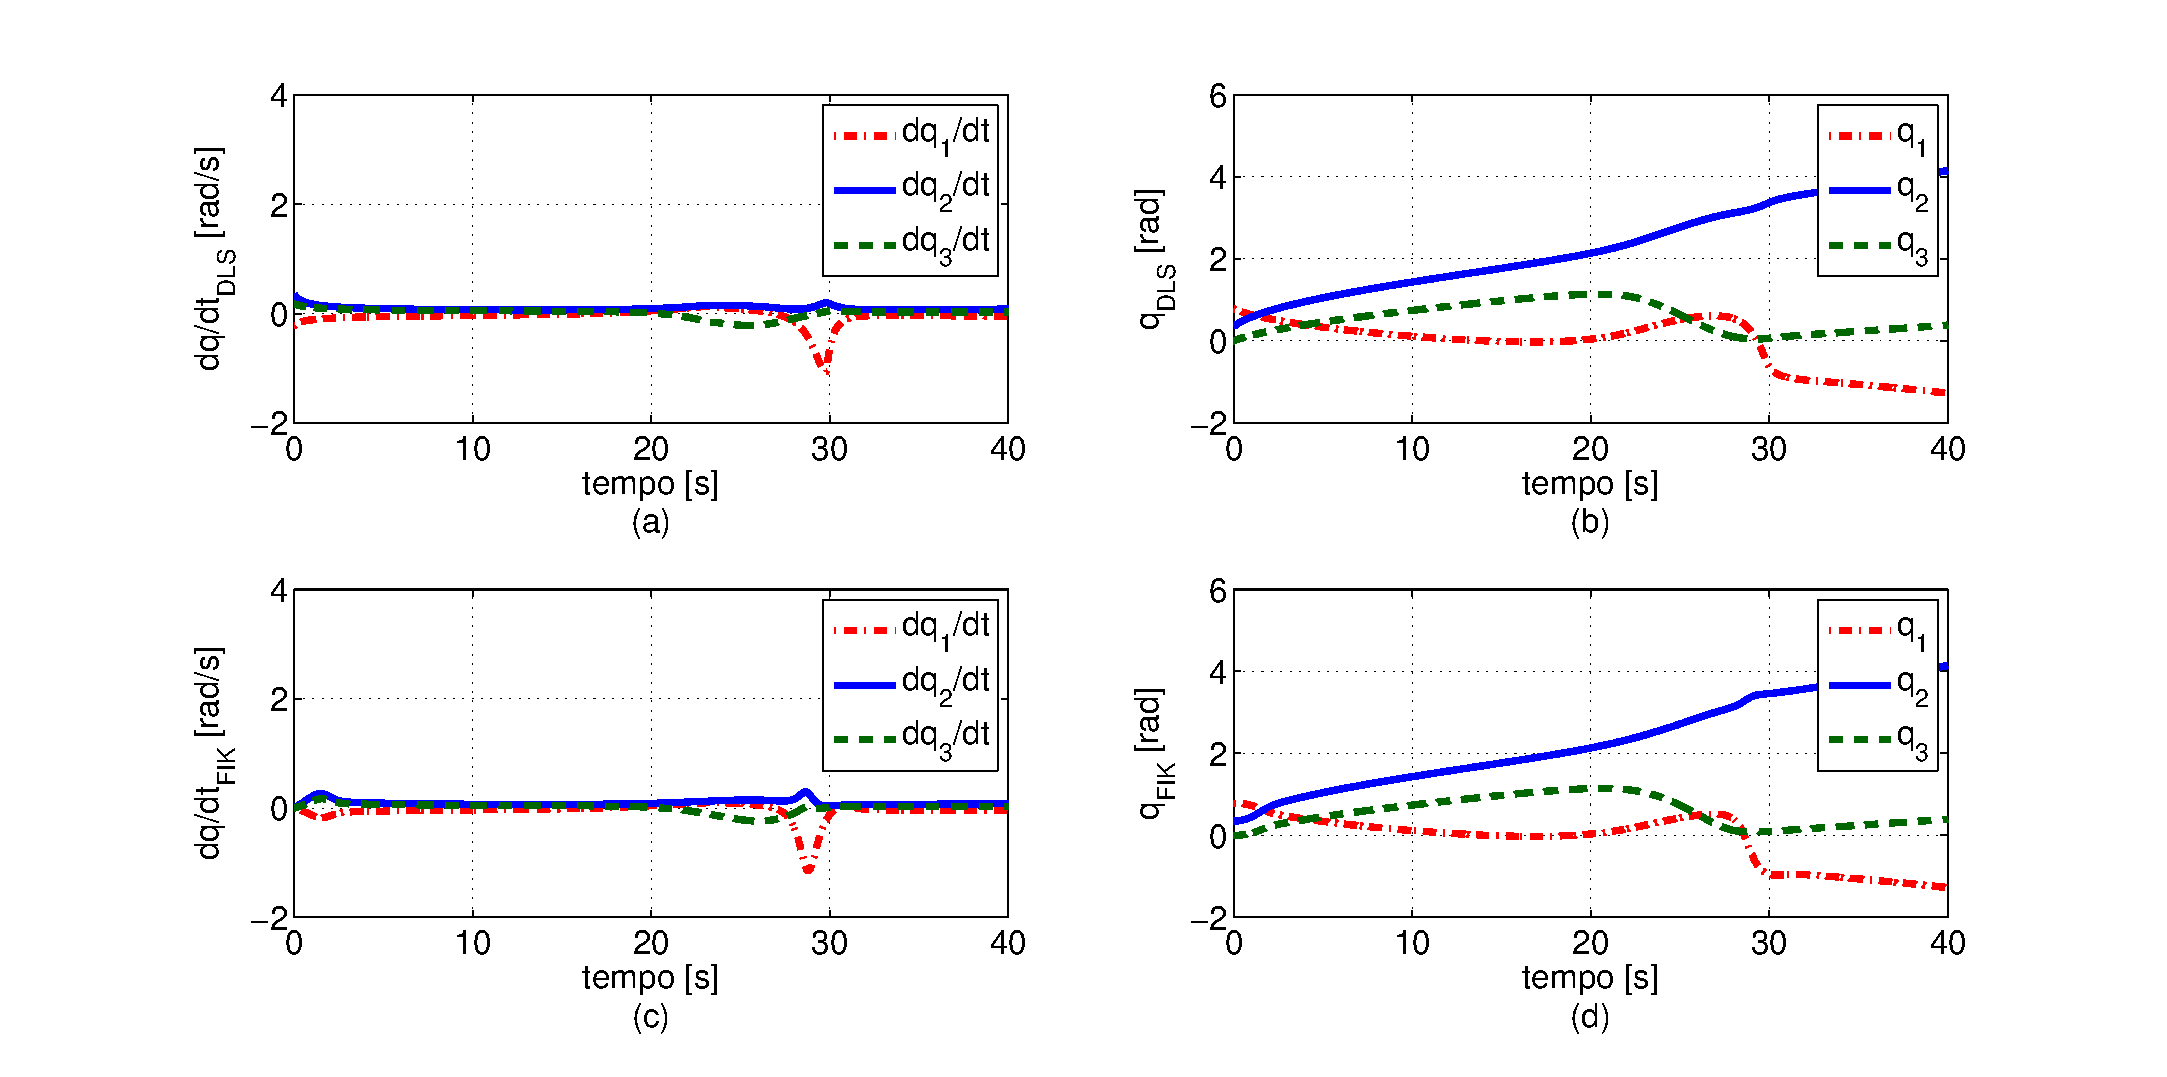
\includegraphics[trim = 2.7cm 0cm 2.7cm 10cm, scale = 0.49]{sim/sim3_data2.eps}\\ %\tiny{\,(b)} \\
\caption{Simula��o \ref{sim::zebra}: (a) normas dos erros; (b) condicionamento; (c) $\dot{\bf q}_p$ e (d) $\dot{\bf q}_o$.}
\label{fig::zebradata}
\end{figure}

Novamente, os erros de postura tendem exponencialmente para zero de acordo com os ganhos ${\boldsymbol \Lambda}_p$ e ${\boldsymbol \Lambda}_o$ (Figura \ref{fig::zebradata}.a). A partir da Figura \ref{fig::zebradata}.b, nota-se que para $t \approx 9s$ o manipulador atinge a vizinhan�a de uma singularidade, resultando em picos de velocidade no espa�o das juntas ( Figuras \ref{fig::zebradata}.c e \ref{fig::zebradata}.d).

\begin{figure}[!htp]
\begin{tabular}{ll}
			\includegraphics[trim = 0cm 0.4cm 0cm 1cm, clip=true, scale = 0.39]{sim/zebra1.eps}& %\tiny{\,(b)} \\
			\includegraphics[trim = 20cm 0.4cm 0cm 1cm, scale = 0.39]{sim/zebra3.eps}\\ %\tiny{\,(b)} \\				
			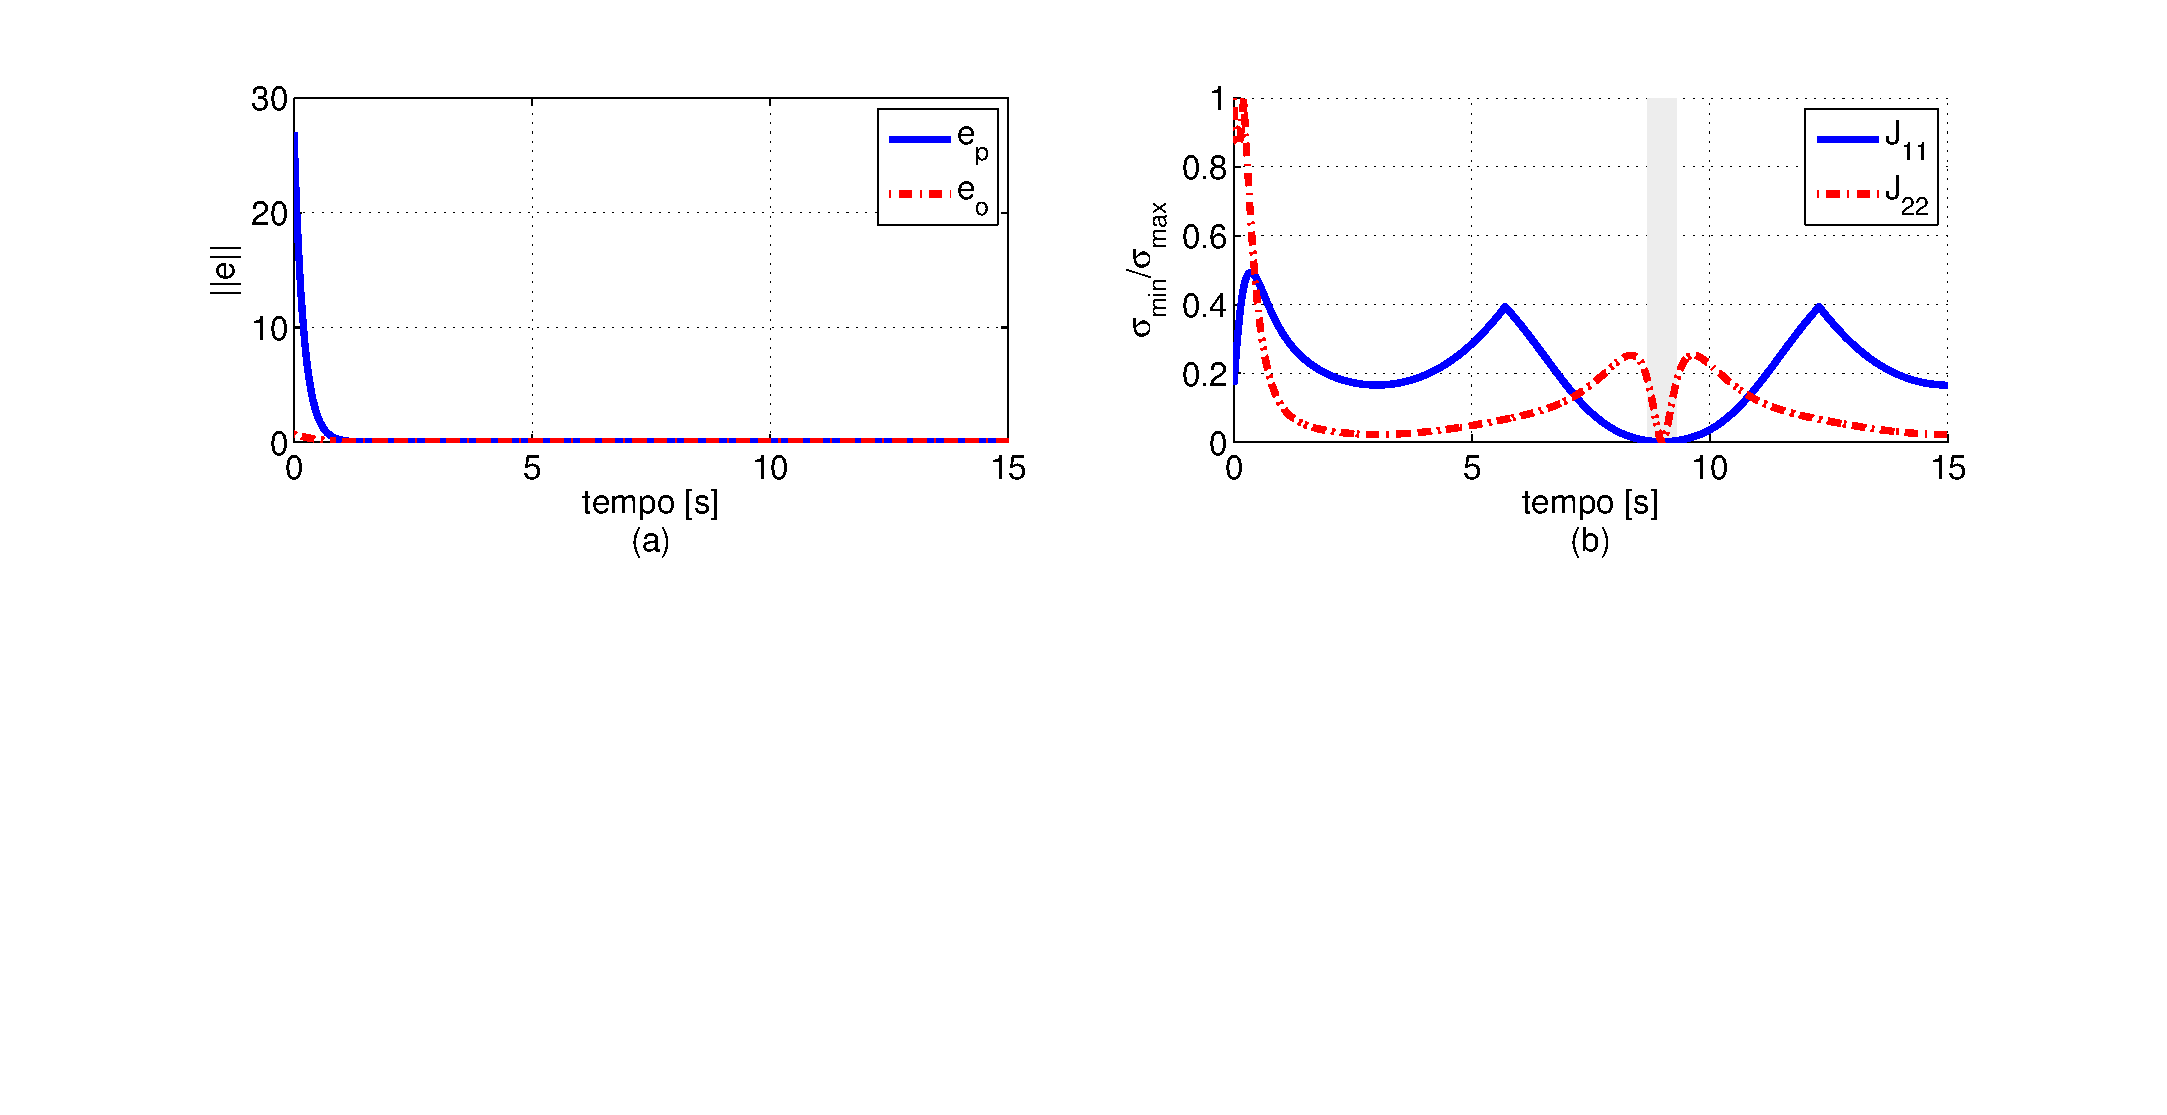
\includegraphics[trim = 2.7cm 9cm 2.7cm 8.6cm, clip=true, scale = 0.49]{sim/indice.eps}\\
\end{tabular}			
\caption{Simula��o \ref{sim::zebra}: Manipulador Zebra-ZERO em diferentes posturas: (a) afastada ($t \approx 1s$) e (b) pr�xima de uma singularidade ($t \approx 9s$).}
\end{figure}


%\begin{figure}[!htp]
  %\centering
 % \label{fig::zebra3d}
%			\begin{tabular}{cc}
%				\includegraphics[trim = 0cm 0cm 0cm 17cm, scale = 0.39]{sim/zebra1.eps}& %\tiny{\,(b)} \\
%				\includegraphics[trim = 0cm 0cm 0cm 17cm, scale = 0.39]{sim/zebra3.eps}\\ %\tiny{\,(b)} \\
%				\end{tabular}
%\caption{Simula��o \ref{sim::zebra}: Manipulador Zebra-ZERO em diferentes posturas: (a) afastada ($t \approx 1s$) e (b) pr�xima de uma singularidade ($t \approx 9s$).}
%\end{figure}

